\subsection{Questão 1 -- Amplificador Fonte-Comum com Transistor NMOS}

\subsubsection{Item 1.a -- Esquemático e Dimensionamento dos Elementos Passivos}

\paragraph{Metodologia}
\vspace{0.2cm}
Conforme especificado no roteiro~\cite{AMP2_1}, propôs-se a topologia de amplificador fonte-comum ilustrada na Figura~\ref{fig:esquematico_nmos}, sendo sua respectiva implementação modelada no ambiente Cadence Virtuoso conforme mostrado na Figura~\ref{fig:esquematico1}. Todas as simulações foram conduzidas no simulador Cadence Spectre (processo TSMC $65\text{ nm}$ CMOS) à temperatura de $40^\circ\text{C}$, com os arquivos de esquemático e simulação organizados no diretório \texttt{\textasciitilde/cadence/tsmc65/Amp2/Lab1} (\texttt{schematic} e \texttt{maestro}).

O transistor \texttt{nmos\_rf} foi dimensionado com largura total $W = 30\ \mu\text{m}$ distribuída em $15$ \textit{fingers} ($2\ \mu\text{m}$ por \textit{finger}) e comprimento de canal igual a quatro vezes o mínimo da tecnologia ($L = 4 \times 60\text{ nm} = 240\text{ nm}$). Na etapa inicial, aplicou-se uma fonte senoidal de entrada de frequência $f = 2\text{ MHz}$ com amplitude de $1\text{ mV}$, resistência de fonte $R_{Sig} = 50\ \Omega$, alimentação $V_{DD} = 1.2\text{ V}$, polarização $V_{Bias}$ e carga $R_L = 2\text{ k}\Omega$. Para determinar os valores mínimos e nominais adequados dos elementos passivos de acoplamento ($C_{in}$, $C_{out}$) e polarização ($L_{in}$, $L_{out}$), realizou-se o cálculo analítico em Python considerando os critérios de reatância na frequência de operação ($X_C = \frac{1}{2\pi f C} \ll R$ para curtos-circuitos AC e $X_L = 2\pi f L \gg R$ para circuitos abertos AC).

\begin{figure}[H]
    \centering
\begin{circuitikz}[american, thick]
    % Estilo para os terminais de alimentação (barra horizontal)
    \tikzset{vrail/.style={draw, line width=1.2pt}}

    % Transistor NMOS principal
    \draw (0,0) node[nmos] (M1) {};
    % Terra do Source
    \draw (M1.S) -- (0,-1.5) node[tground] {};

    % Indutor de dreno e alimentação V_DD
    \draw (M1.D) -- (0,1.2) to[L] (0,2.8) -- (0,3.2);
    \draw[vrail] (-0.4,3.2) -- (0.4,3.2) node[midway, above] {$\mathrm{V_{DD}}$};

    % Ramo da esquerda (Gate, Bias, v_in, C_in, R_Sig, v_Sig)
    \draw (M1.G) -- (-1.5,0) coordinate (N_bias);
    
    % Indutor de polarização e V_Bias
    \draw (N_bias) to[L] (-1.5,2.2) -- (-1.5,2.6);
    \draw[vrail] (-1.9,2.6) -- (-1.1,2.6) node[midway, above] {$\mathrm{V_{Bias}}$};

    % Nó v_in
    \draw (N_bias) -- (-2.5,0) coordinate (N_vin);
    \draw (N_vin) -- (-2.5,0.6) node[ocirc] {} node[above, blue] {$\mathcal{V}_{in}$};

    % Capacitor de acoplamento de entrada
    \draw (N_vin) to[C] (-3.8,0) coordinate (N_cin);

    % Parte em cinza da entrada (R_Sig e v_Sig)
    \begin{scope}[color=black]
        \draw (N_cin) to[R, l_=$\mathcal{R}_{Sig}$] (-5.3,0)
              to[V, v=$\mathcal{V}_{Sig}$] (-5.3,-1.5) node[tground] {};
    \end{scope}

    % Ramo da direita (Dreno, C_out, R_L, v_out)
    \draw (M1.D) -- (0,1.0) coordinate (N_drain);
    \draw (N_drain) to[C] (2.2,1.0) coordinate (N_cout);

    % Parte em cinza da saída (R_L)
    \begin{scope}[color=black]
        \draw (N_cout) to[R, l=$\mathcal{R}_{L}$] (2.2,-0.8) node[tground] {};
    \end{scope}

    % Nó v_out
    \draw (N_cout) -- (3.2,1.0) node[ocirc] {} node[above, blue] {$\mathcal{V}_{out}$};

\end{circuitikz}
    \caption{Esquemático do amplificador fonte-comum com transistor NMOS.}
    \label{fig:esquematico_nmos}
\end{figure}

\begin{figure}[H]
    \centering
    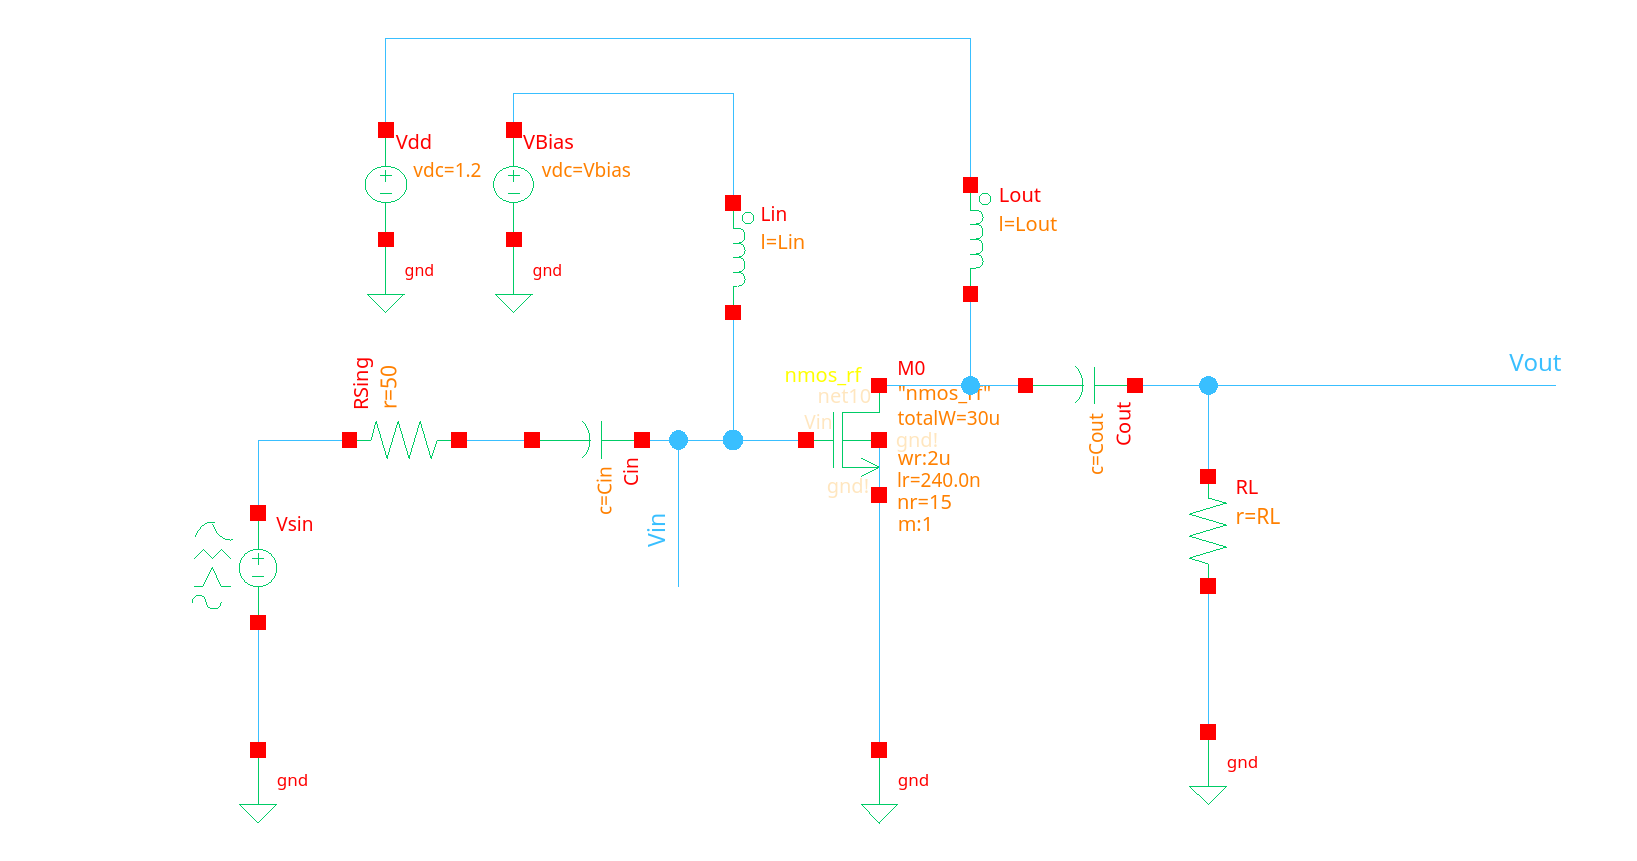
\includegraphics[width=0.82\textwidth]{Geral/Fig/Esquematico 1.png}
    \caption{Esquemático do amplificador fonte-comum com transistor NMOS, modelado no Cadence.}
    \label{fig:esquematico1}
\end{figure}

\paragraph{Resultados}
\vspace{0.2cm}
A Tabela~\ref{tab:passivos} sintetiza os valores mínimos obtidos via cálculo em Python para a frequência de $2\text{ MHz}$, juntamente com os valores nominais adotados no esquemático do Cadence para garantir o regime ideal de pequenos sinais.

\begin{table}[H]
    \centering
    \caption{Dimensionamento dos componentes passivos para $f = 2\text{ MHz}$.}
    \label{tab:passivos}
    \begin{tabular}{lcc}
        \hline
        \textbf{Componente} & \textbf{Mínimo Calculado} & \textbf{Valor Adotado} \\
        \hline
        $C_{in}$ & $15.92\text{ nF}$ & $1\ \mu\text{F}$ \\
        $C_{out}$ & $3.98\text{ nF}$ & $1\ \mu\text{F}$ \\
        $L_{in}$ & $0.40\text{ mH}$ & $10\text{ mH}$ \\
        $L_{out}$ (com $R_L = 2\text{ k}\Omega$) & $15.92\text{ mH}$ & $100\text{ mH}$ \\
        $L_{out}$ (circuito aberto) & $99.47\text{ mH}$ & $100\text{ mH}$ \\
        \hline
    \end{tabular}
\end{table}

\paragraph{Conclusão}
\vspace{0.2cm}
A adoção de capacitores de $1\ \mu\text{F}$ ($X_C \approx 79.6\ \text{m}\Omega$) e indutores de $10\text{ mH}$ ($X_{Lin} \approx 125.7\ \text{k}\Omega$) e $100\text{ mH}$ ($X_{Lout} \approx 1.257\ \text{M}\Omega$) isola completamente os pontos de polarização DC dos sinais AC de $2\text{ MHz}$, eliminando divisores capacitivos e desvios de corrente AC tanto na condição com carga quanto em circuito aberto.

\subsubsection{Item 1.b -- Simulação Transiente e Ganho de Tensão}

\paragraph{Metodologia}
\vspace{0.2cm}
Após a conclusão do esquemático, criou-se a vista \texttt{maestro} (teste \texttt{Amp2\_Lab1}), na qual foi executada uma análise transiente (\texttt{tran}) no ponto de polarização em saturação ($V_{Bias} \approx 780\text{ mV}$) com carga $R_L = 2\text{ k}\Omega$. Para eliminar a influência do transitório inicial de carga dos elementos reativos ($C$ e $L$), o ganho de tensão de pequenos sinais foi avaliado em regime permanente na janela de $2\ \mu\text{s}$ a $5\ \mu\text{s}$ ($6$ ciclos completos do sinal de $f = 2\text{ MHz}$, cujo período é $T = 1/f = 0.5\ \mu\text{s}$) por meio da expressão \texttt{Ganho\_Av} configurada na tabela de saídas (\textit{Outputs Setup}) do ADE Explorer (onde \texttt{/net1} corresponde ao nó de saída \texttt{/Vout}):
\begin{equation}
    |A_v| = \frac{\text{peakToPeak}(\text{clip}(V_T(\text{''/net1''}), 2\mu, 5\mu))}{\text{peakToPeak}(\text{clip}(V_T(\text{''/Vin''}), 2\mu, 5\mu))}
\end{equation}
Adicionalmente, configurou-se a razão instantânea ponto a ponto entre os sinais totais de saída e entrada para verificar o comportamento temporal do estágio:
\begin{equation}
    A_{v,\text{inst}}(t) = \frac{V_T(\text{''/net1''})}{V_T(\text{''/Vin''})}
\end{equation}

\paragraph{Resultados}
\vspace{0.2cm}
Analiticamente, na frequência de $2\text{ MHz}$, os capacitores atuam como curtos-circuitos e os indutores como circuitos abertos ($v_{gs} = v_{in}$). Aplicando a Lei das Correntes de Kirchhoff (LCK) no nó de dreno, obtém-se a expressão algébrica do ganho de tensão de pequenos sinais:
\begin{equation}
    A_v = \frac{v_{out}}{v_{in}} = -g_m \cdot (r_o \parallel R_L) = -g_m \cdot \left(\frac{r_o \cdot R_L}{r_o + R_L}\right)
\end{equation}

Substituindo a resistência de carga $R_L = 2\text{ k}\Omega$ e os parâmetros intrínsecos de pequenos sinais do transistor \texttt{nmos\_rf} no ponto de polarização ($g_m = 8.42\text{ mS}$ e $r_o = 25\text{ k}\Omega$ no dimensionamento analítico, ou $g_m = 10.42\text{ mS}$ e $r_o = 5.761\text{ k}\Omega$ extraídos via \texttt{OP("/M0")}), obtém-se o ganho teórico assintótico entre $15.47\text{ V/V}$ e $15.59\text{ V/V}$:
\begin{equation}
    |A_{v,\text{teórico}}| = 8.42\text{ mS} \times \left(\frac{25\text{ k}\Omega \times 2\text{ k}\Omega}{25\text{ k}\Omega + 2\text{ k}\Omega}\right) = 15.59\text{ V/V}
\end{equation}

Para provar que os resultados apresentados nos gráficos do Cadence ViVA estão matematicamente corretos, confrontaram-se as equações teóricas com as leituras diretas das formas de onda:
\begin{enumerate}
    \item \textbf{Validação do Gráfico Transiente (Figura~\ref{fig:transiente_vout_vin}):} Com uma excitação senoidal de entrada de amplitude $1.0\text{ mV}$ ($\Delta V_{in,\text{pp}} = 2.0\text{ mV}$) e período $T = 500.0\text{ ns}$ ($f = 2.0\text{ MHz}$), a saída apresenta excursão pico a pico de $\Delta V_{out,\text{pp}} = 30.98\text{ mV}$ (amplitude de $15.49\text{ mV}$). A razão direta entre essas amplitudes fornece:
    \begin{equation}
        |A_{v,\text{gráfico}}| = \frac{\Delta V_{out,\text{pp}}}{\Delta V_{in,\text{pp}}} = \frac{30.98\text{ mV}}{2.0\text{ mV}} = 15.49\text{ V/V}
    \end{equation}
    Esse valor coincide exatamente com a leitura automatizada \texttt{Ganho\_Av = 15.49} exibida no gráfico e apresenta desvio de apenas $0.64\%$ em relação ao ganho teórico assintótico ($15.59\text{ V/V}$), validando a expressão da Calculator.

    \item \textbf{Validação da Razão Instantânea e Inversão de Fase (Figura~\ref{fig:av_inst}):} Como a expressão \texttt{Av\_Inst} divide o sinal total de saída $V_{out}(t)$ (nível DC nulo devido a $C_{out}$) pelo sinal total de entrada $V_{in}(t) = V_{DC} + v_{in}(t)$ (onde $V_{DC} \approx 780\text{ mV}$ e $v_{in,\text{pico}} = 1\text{ mV}$), e sendo o estágio fonte-comum \textbf{inversor} ($180^\circ$ de defasagem), os extremos teóricos da curva devem ocorrer nos picos opostos de $V_{in}$ e $V_{out}$:
    \begin{equation}
        A_{v,\text{inst(máx)}} = \frac{+15.40\text{ mV}}{780\text{ mV} - 1\text{ mV}} = +19.77\text{ m} \qquad \text{e} \qquad A_{v,\text{inst(mín)}} = \frac{-15.34\text{ mV}}{780\text{ mV} + 1\text{ mV}} = -19.64\text{ m}
    \end{equation}
    Esses valores teóricos coincidem exatamente com os marcadores medidos no gráfico da Figura~\ref{fig:av_inst} (\texttt{M1 = 19.7699m} e \texttt{M2 = -19.6366m}, com período $T = 499.8\text{ ns}$), comprovando matematicamente tanto a inversão de fase do amplificador quanto a exatidão numérica de ambas as curvas simuladas.
\end{enumerate}

\begin{figure}[H]
    \centering
    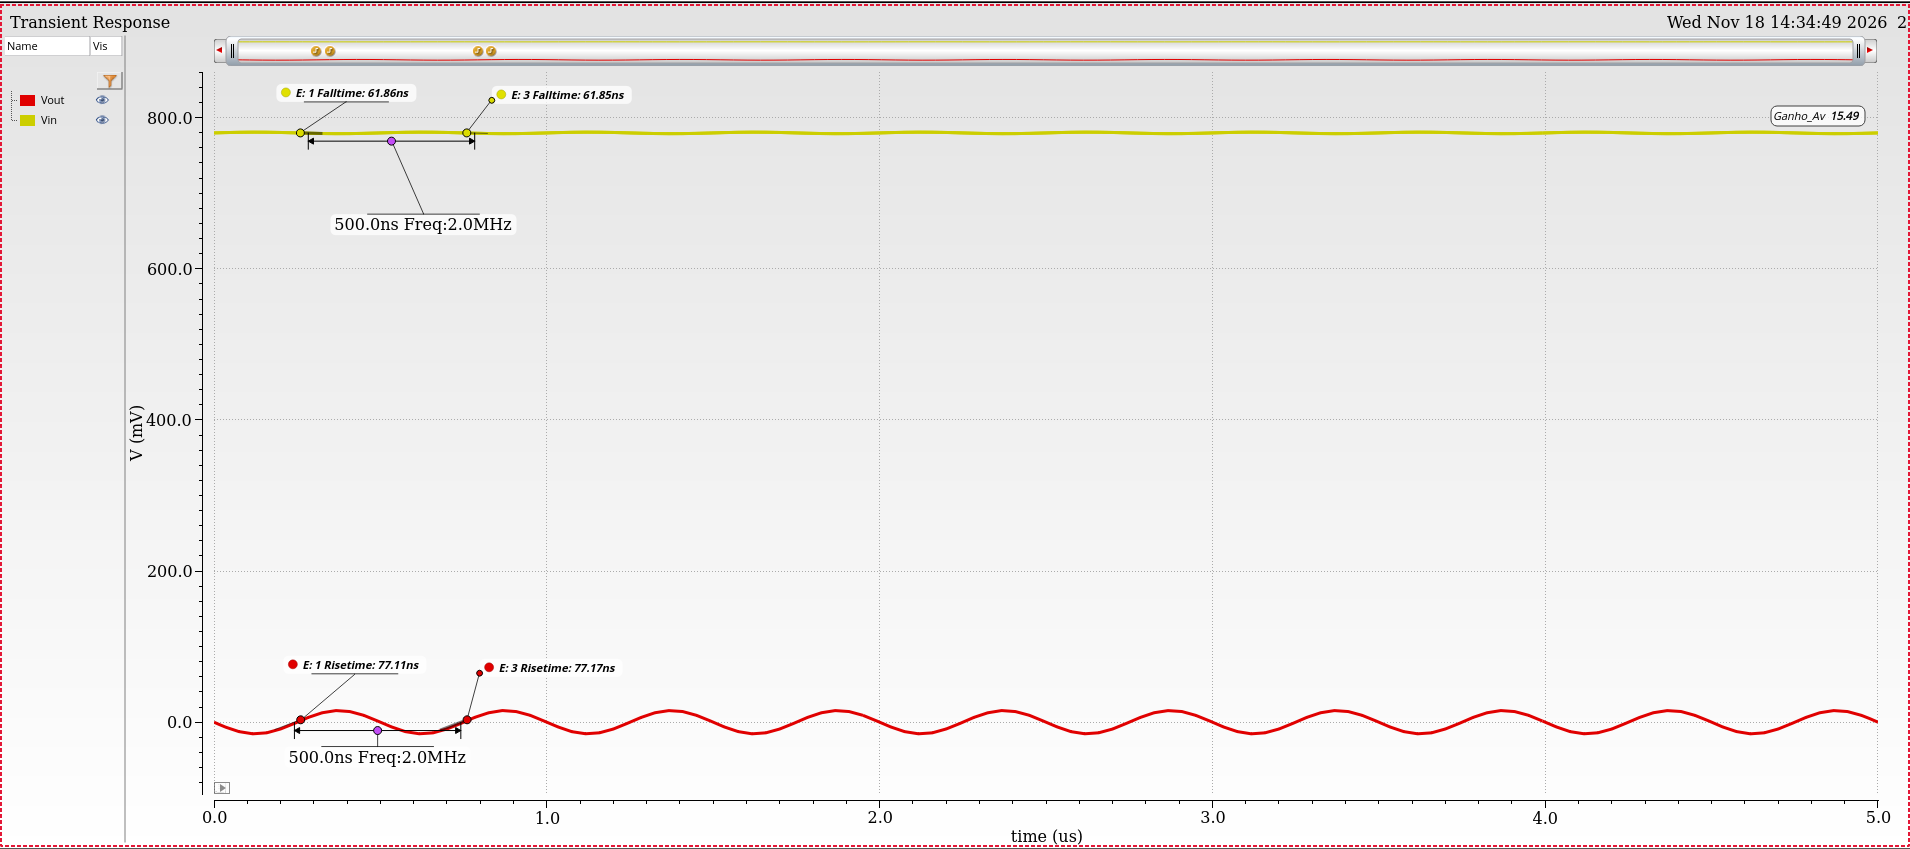
\includegraphics[width=0.92\textwidth]{Geral/Fig/transiente_vout_vin.png}
    \caption{Formas de onda transientes de $V_{in}$ e $V_{out}$ em $f = 2.0\text{ MHz}$ ($T = 500\text{ ns}$) e valor calculado de $|A_v| = 15.49\text{ V/V}$.}
    \label{fig:transiente_vout_vin}
\end{figure}

\begin{figure}[H]
    \centering
    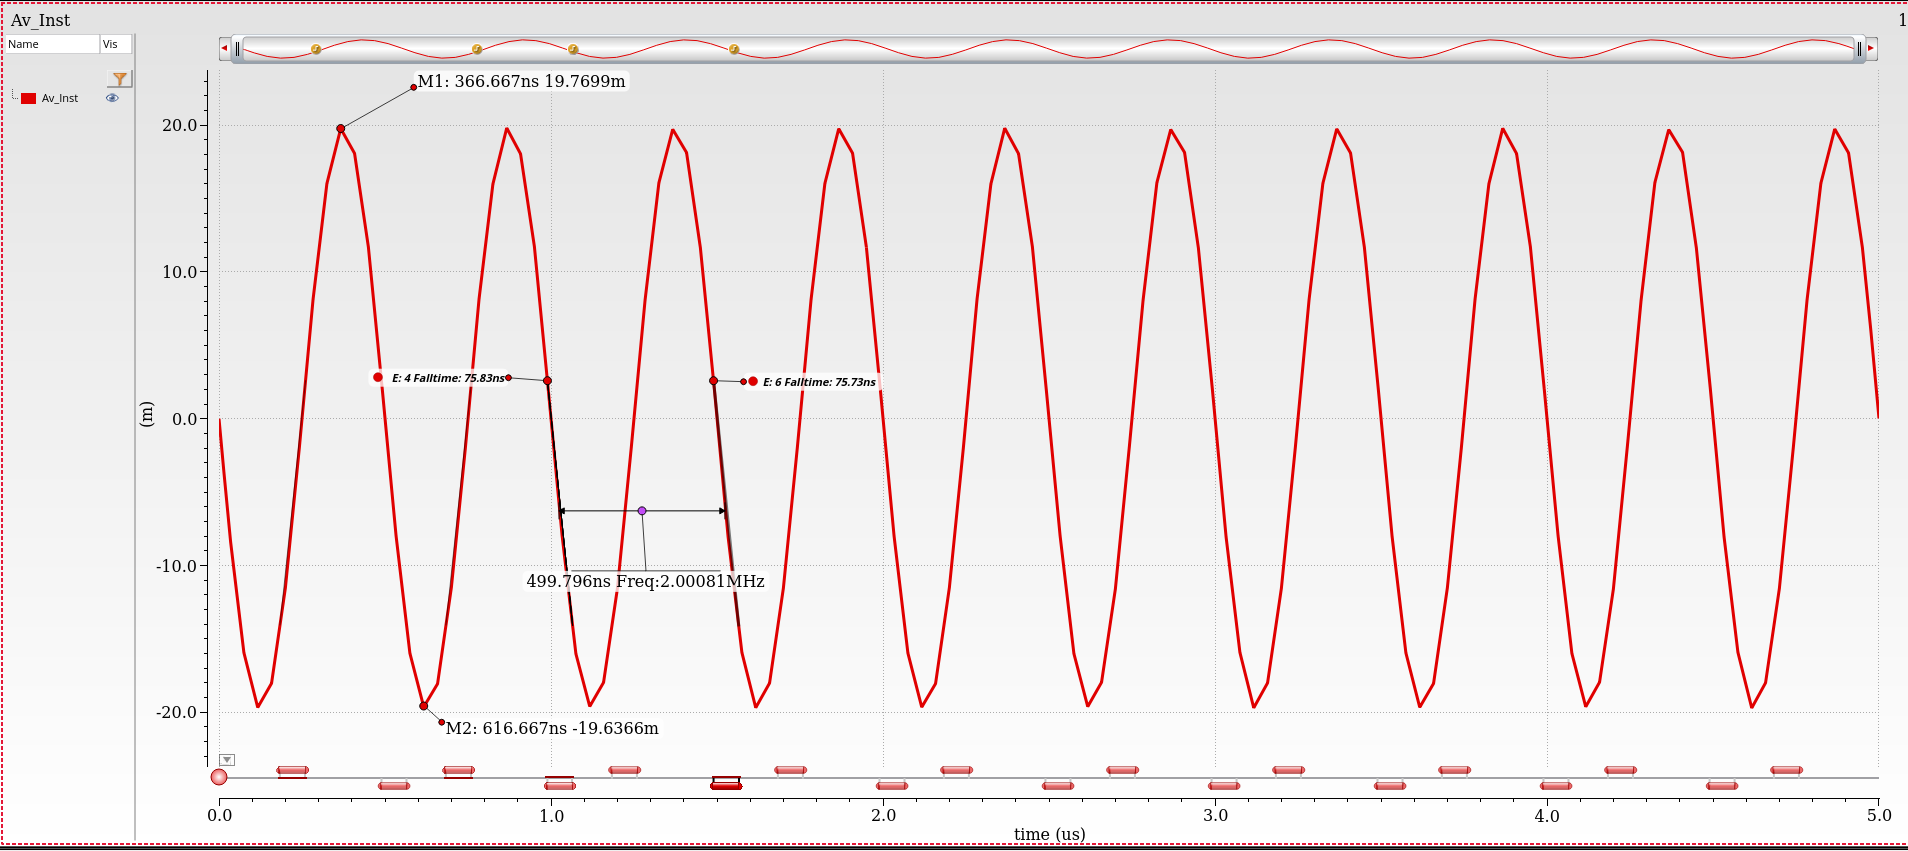
\includegraphics[width=0.92\textwidth]{Geral/Fig/av_inst.png}
    \caption{Forma de onda da razão instantânea \texttt{Av\_Inst} ($V_T(\text{''/Vout''})/V_T(\text{''/Vin''})$), evidenciando o período de $499.8\text{ ns}$ ($f \approx 2.0\text{ MHz}$) e os marcadores \texttt{M1 = 19.77m} e \texttt{M2 = -19.64m}.}
    \label{fig:av_inst}
\end{figure}

\paragraph{Conclusão}
\vspace{0.2cm}
A comprovação numérica entre as equações analíticas e as leituras diretas dos marcadores nos gráficos confirma que o estágio fonte-comum opera linearmente na saturação com ganho inversor de $|A_v| = 15.49\text{ V/V}$ (erro de $0.64\%$ frente ao modelo teórico assintótico). Além disso, a demonstração matemática dos picos de \texttt{Av\_Inst} ($+19.77\text{ m}$ e $-19.64\text{ m}$) prova que a expressão automatizada \texttt{Ganho\_Av} com a função \texttt{peakToPeak} está correta e é indispensável para isolar a excursão AC do nível DC de polarização nas análises subsequentes.

\subsubsection{Item 1.c -- Determinação do Ganho em Circuito Aberto ($A_{vo} \approx 60$)}

\paragraph{Metodologia}
\vspace{0.2cm}
Removeu-se a carga externa ($R_L \to \infty$) para avaliar o ganho de tensão intrínseco em circuito aberto ($A_{vo} = -g_m \cdot r_o$). Na tabela de saídas do ADE Explorer, definiu-se a expressão \texttt{Ganho\_Av} na janela estabilizada de $2\ \mu\text{s}$ a $5\ \mu\text{s}$ (além da razão instantânea \texttt{Av\_Inst = VT("/Vout") / VT("/Vin")}):
\begin{equation}
    |A_{vo}| = \frac{\text{peakToPeak}(\text{clip}(V_T(\text{''/Vout''}), 2\mu, 5\mu))}{\text{peakToPeak}(\text{clip}(V_T(\text{''/Vin''}), 2\mu, 5\mu))}
\end{equation}
Para determinar o valor de $V_{Bias}$ ($0 < V_{Bias} \le V_{DD}$) que resulta em $|A_{vo}| \approx 60\text{ V/V}$, realizou-se primeiramente uma varredura paramétrica ampla de $0\text{ mV}$ a $1200\text{ mV}$ com passo linear de $100\text{ mV}$, seguida de uma inspeção detalhada nas regiões de cruzamento e de uma varredura fina com passo de $0.5\text{ mV}$ na faixa de operação estável.

\paragraph{Resultados}
\vspace{0.2cm}
Na varredura ampla (Figura~\ref{fig:varredura_geral}), observou-se que a curva cruza o patamar de $60\text{ V/V}$ em duas regiões distintas: uma na faixa inferior, em torno de $V_{Bias} = 278.27\text{ mV}$ (situada entre $200\text{ mV}$, com ganho de $10.7\text{ V/V}$, e $300\text{ mV}$, com ganho de $73.68\text{ V/V}$), e outra na faixa superior, entre $700\text{ mV}$ (com ganho de $64.41\text{ V/V}$) e $800\text{ mV}$ (com ganho de $58.65\text{ V/V}$). Ao analisar detalhadamente a região inferior entre $200\text{ mV}$ e $300\text{ mV}$ (Figura~\ref{fig:varredura_inferior}), verificaram-se múltiplos cruzamentos instáveis ($274.27\text{ mV}$, $291.61\text{ mV}$ e $295.97\text{ mV}$) decorrentes da operação do transistor em corte/inversão fraca ($V_{GS} < V_{th}$). Na varredura fina entre $700\text{ mV}$ e $800\text{ mV}$ com passo de $0.5\text{ mV}$ (Figura~\ref{fig:varredura_fina}), identificou-se o cruzamento exato em $V_{Bias} = 779.8\text{ mV}$ (próximo ao valor interpolado de $776.54\text{ mV}$) para $|A_{vo}| = 60\text{ V/V}$.

\begin{figure}[H]
    \centering
    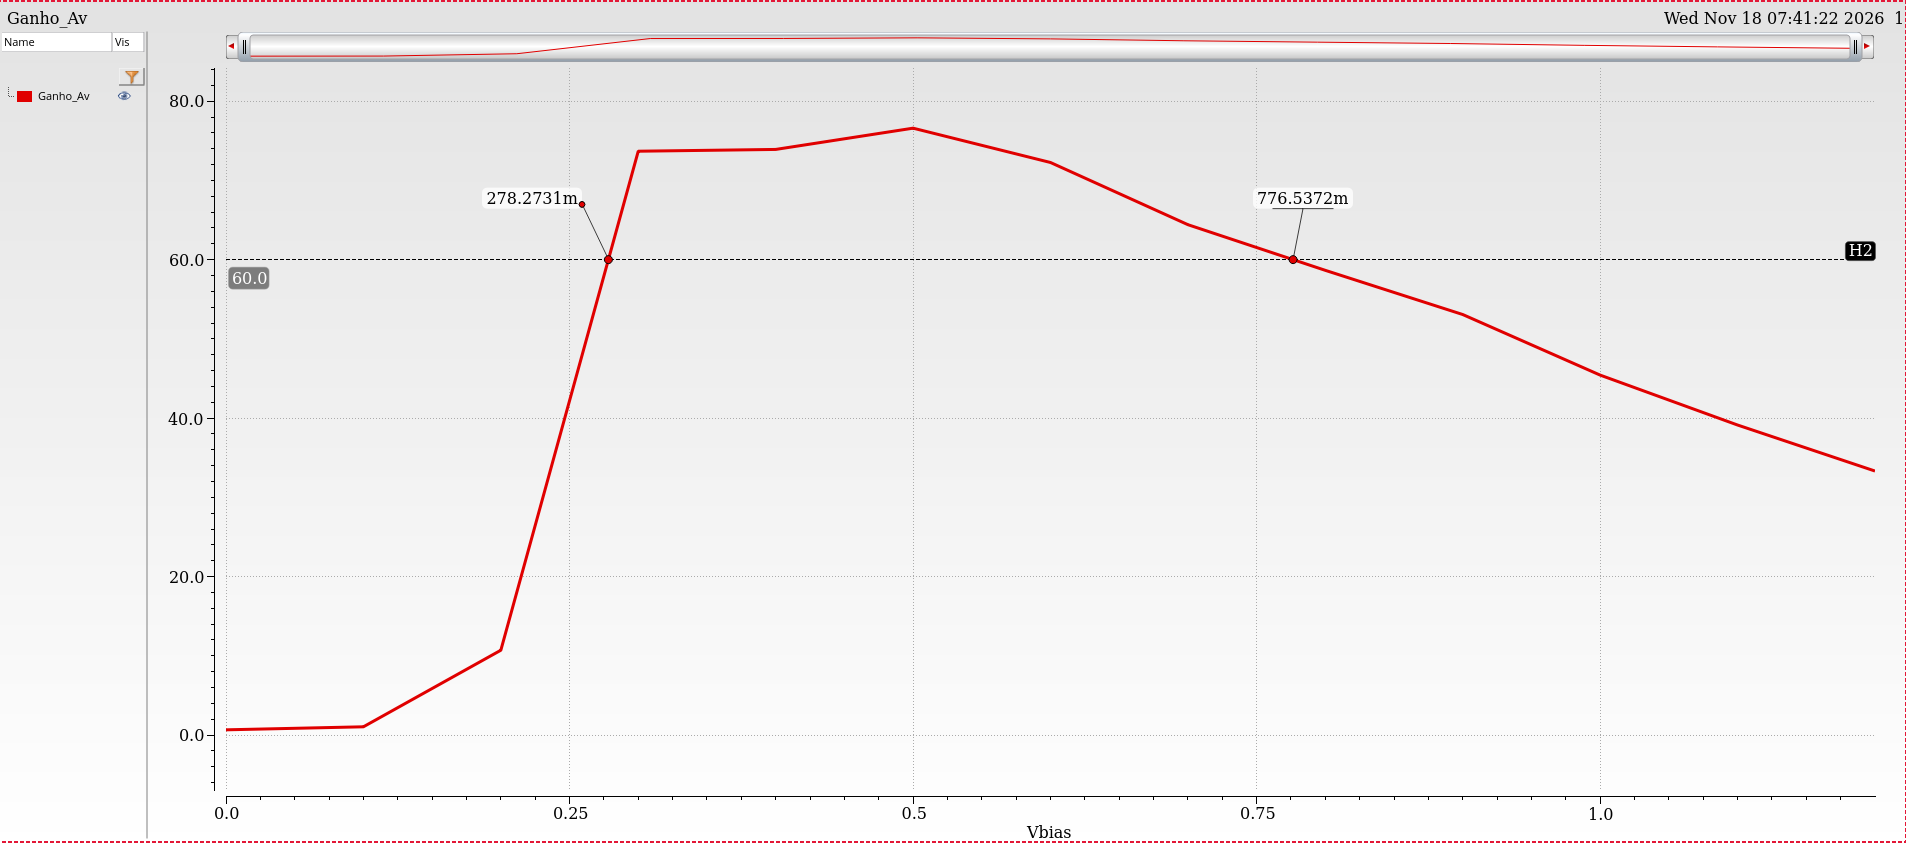
\includegraphics[width=0.80\textwidth]{Geral/Fig/varredura_0_1200m.png}
    \caption{Varredura paramétrica ampla de $V_{Bias}$ ($0$ a $1200\text{ mV}$) mostrando os dois pontos de cruzamento para $|A_{vo}| = 60\text{ V/V}$.}
    \label{fig:varredura_geral}
\end{figure}

\begin{figure}[H]
    \centering
    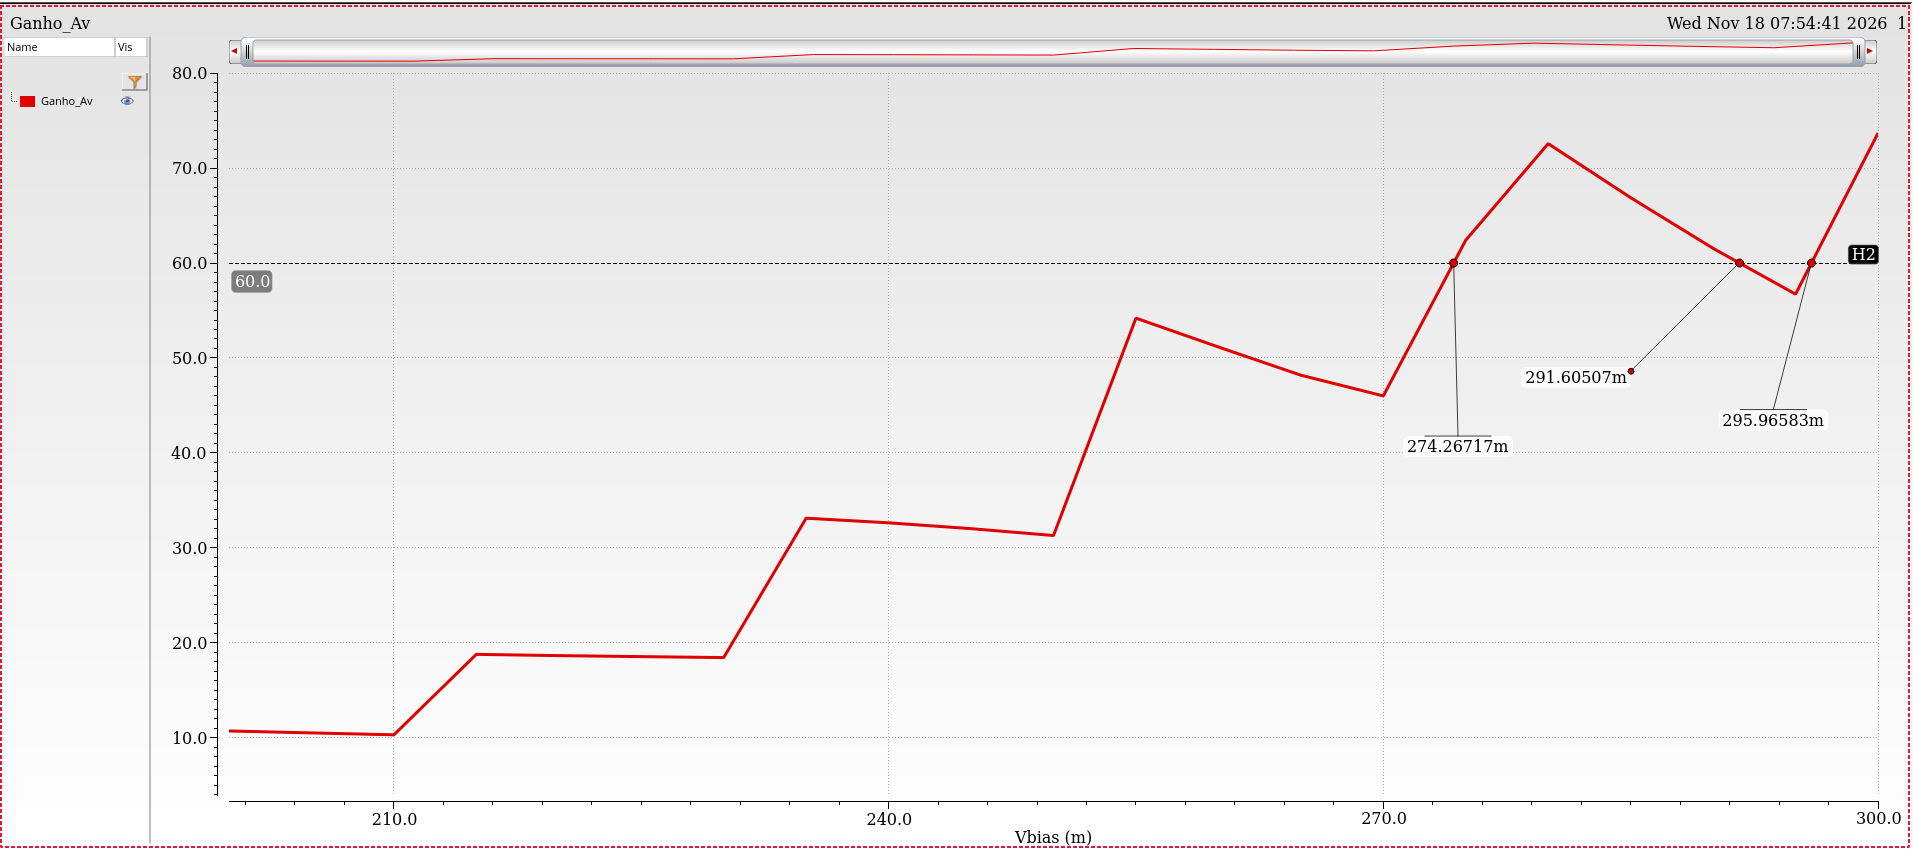
\includegraphics[width=0.80\textwidth]{Geral/Fig/varredura_200_300m.png}
    \caption{Detalhe da varredura de $V_{Bias}$ entre $200\text{ mV}$ e $300\text{ mV}$, evidenciando as oscilações numéricas na região de inversão fraca.}
    \label{fig:varredura_inferior}
\end{figure}

\begin{figure}[H]
    \centering
    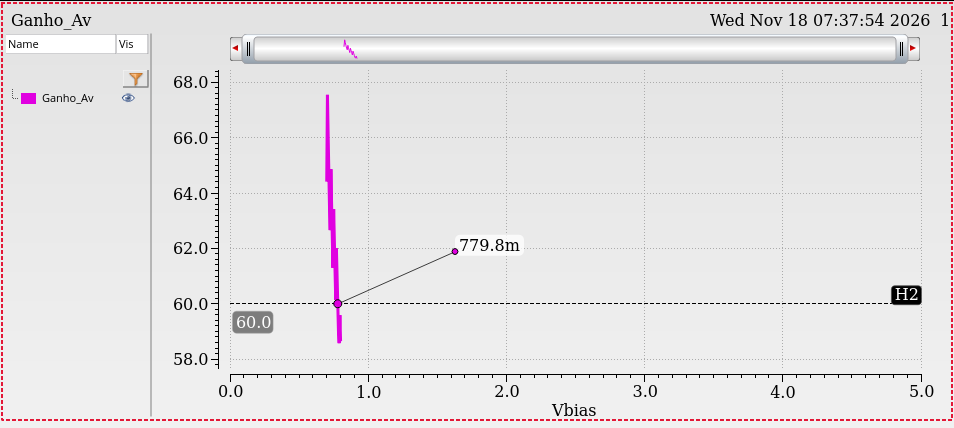
\includegraphics[width=0.80\textwidth]{Geral/Fig/varredura_700_800m.png}
    \caption{Varredura fina de $V_{Bias}$ na faixa superior para determinação exata do ponto de $|A_{vo}| = 60\text{ V/V}$.}
    \label{fig:varredura_fina}
\end{figure}

\paragraph{Conclusão}
\vspace{0.2cm}
Adotou-se a tensão de polarização $V_{Bias} = 779.8\text{ mV}$ ($\approx 777\text{ mV}$ a $780\text{ mV}$), pois nesse ponto o dispositivo opera plenamente em \textbf{saturação (inversão forte)}, superando com folga a tensão de limiar do NMOS ($V_{th} \approx 0.4\text{ V}$). Ao contrário da região inferior de sublimiar (onde a corrente de dreno quase nula provoca atraso na acomodação transitória e imprecisões numéricas), a polarização em $779.8\text{ mV}$ garante canal plenamente formado, resposta linear estável, elevada transcondutância ($g_m$) e o cumprimento da restrição $0 < V_{Bias} \le V_{DD}$.

\subsubsection{Item 1.d -- Transcondutância em Curto-Circuito ($G_m$) e Comparação com o Ponto DC}

\paragraph{Metodologia}
\vspace{0.2cm}
Mantendo $V_{Bias} = 779.8\text{ mV}$, curto-circuitou-se a saída do amplificador conectando o terminal direito de $C_{out}$ diretamente ao terra ($v_{out} = 0\text{ V}$). Executou-se a simulação transiente (\texttt{tran}) para registrar as formas de onda temporais da corrente AC de curto-circuito ($i_{out}$, em $\mu\text{A}$) e da tensão de porta ($v_{in}$, em $\text{mV}$), separando-as em dois painéis no visualizador ViVA e gerando o gráfico de transferência $I \times V$ (\texttt{Iout\_Vin}) via função \textit{Y vs Y} (\texttt{IT("/Cout/MINUS")} no eixo Y em função de \texttt{VT("/Vin")} no eixo X) para extração gráfica do coeficiente angular via marcador diferencial.

Para a extração automatizada no Cadence ADE Explorer, configuraram-se as expressões listadas na Tabela~\ref{tab:expressoes_ade}, mantendo preservadas (porém desativadas) as expressões de tensão da etapa anterior (\texttt{Ganho\_Av} e \texttt{Av\_Inst}) e ativando as equações de curto-circuito (\texttt{Gm\_Tran} e \texttt{ro\_tran}) e de ponto de operação estático (\texttt{gm\_dc} e \texttt{ro\_dc}) obtidas mediante simulação \texttt{dc} com \textit{Save DC Operating Point} habilitado sobre o transistor \texttt{nmos\_rf} (\texttt{M0}).

\begin{table}[H]
    \centering
    \caption{Expressões configuradas no Cadence ADE Explorer nas etapas de ensaio do estágio NMOS.}
    \label{tab:expressoes_ade}
    \small
    \begin{tabular}{l l p{7.4cm}}
        \hline
        \textbf{Nome} & \textbf{Etapa do Ensaio} & \textbf{Expressão (\textit{Details})} \\
        \hline
        \texttt{Ganho\_Av} & Aberto / Carga $R_L$ & \texttt{peakToPeak(clip(VT("/Vout") 2e-06 5e-06)) / peakToPeak(clip(VT("/Vin") 2e-06 5e-06))} \\
        \texttt{Av\_Inst} & Aberto / Carga $R_L$ & \texttt{VT("/Vout") / VT("/Vin")} \\
        \texttt{Gm\_Tran} & Curto-Circuito & \texttt{peakToPeak(clip(IT("/Cout/MINUS") 2e-06 5e-06)) / peakToPeak(clip(VT("/Vin") 2e-06 5e-06))} \\
        \texttt{ro\_tran} & Curto-Circuito & \texttt{60 / Gm\_Tran} \\
        \texttt{gm\_dc} & Ponto DC & \texttt{OP("/M0" "gm")} \\
        \texttt{ro\_dc} & Ponto DC & \texttt{1 / OP("/M0" "gds")} \\
        \hline
    \end{tabular}
\end{table}

\paragraph{Resultados}
\vspace{0.2cm}
Conforme observado no gráfico à direita da Figura~\ref{fig:transiente_gm_nmos}, a característica de transferência $i_{out} \times v_{in}$ (\texttt{Iout\_Vin}) apresenta comportamento estritamente linear, cujo coeficiente angular fornece diretamente o módulo da transcondutância em curto-circuito ($|G_m|$), apresentando inclinação positiva de $+10.26\text{ mA/V}$ devido à convenção do terminal de saída do capacitor (\texttt{IT("/Cout/MINUS")}, corrente fluindo do capacitor para o terra). Por meio da ferramenta de marcador diferencial (\textit{Delta Marker}) do Cadence ViVA ($\Delta v_{in} = 755.79\ \mu\text{V}$ e $\Delta i_{out} = 7.756\ \mu\text{A}$), extraiu-se $|G_m| = 10.2626\text{ mA/V}$ ($\approx 10.26\text{ mS}$), valor confirmado exatamente pela expressão \texttt{Gm\_Tran} avaliada na Calculator:
\begin{equation}
    |G_m| = \left.\frac{i_{out}}{v_{in}}\right|_{v_{out}=0} = 10.26\text{ mS}
\end{equation}

\begin{figure}[H]
    \centering
    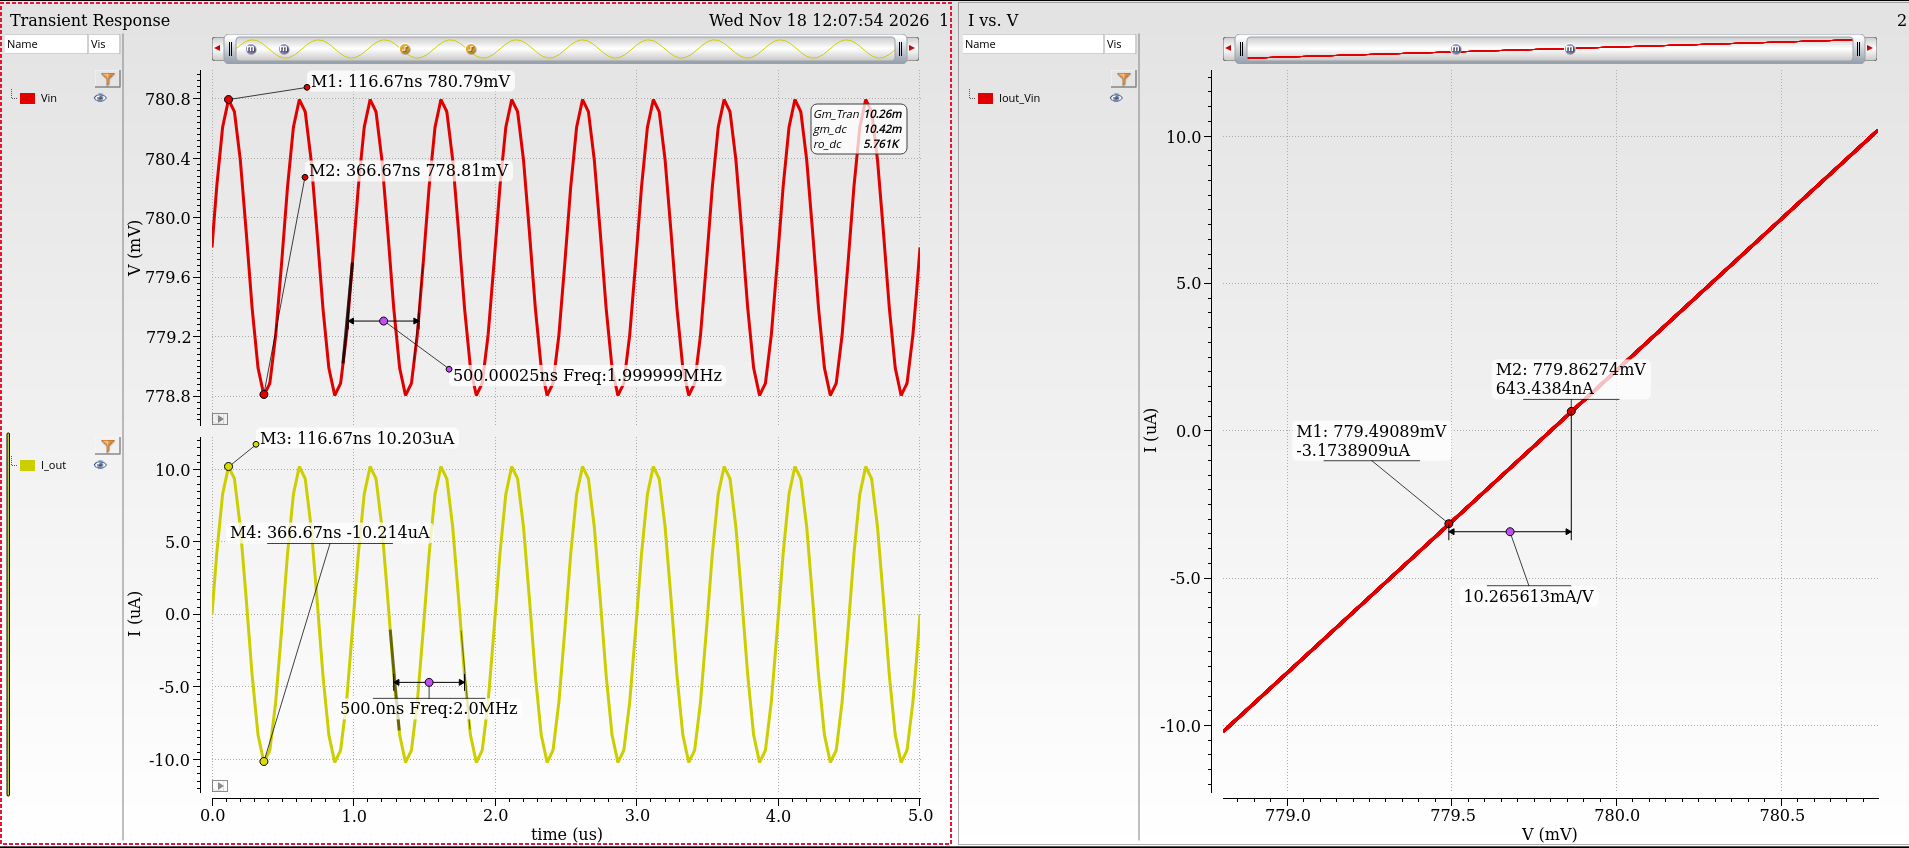
\includegraphics[width=0.92\textwidth]{Geral/Fig/transiente_gm_nmos.png}
    \caption{À esquerda: formas de onda transientes de $v_{in}$ e $i_{out}$ em curto-circuito para $V_{Bias} = 779.8\text{ mV}$. À direita: característica de transferência $i_{out} \times v_{in}$ (\texttt{Iout\_Vin}) linear com coeficiente angular de $10.26\text{ mA/V}$.}
    \label{fig:transiente_gm_nmos}
\end{figure}

Como os passivos são ideais em $2\text{ MHz}$, tem-se $g_m \approx |G_m| = 10.26\text{ mS}$, e a resistência de saída intrínseca calculada via \texttt{ro\_tran} resulta em:
\begin{equation}
    r_{o,\text{tran}} = \frac{|A_{vo}|}{|G_m|} = \frac{60}{10.26\text{ mS}} = 5.845\text{ k}\Omega
\end{equation}
Na análise de ponto de operação DC sobre \texttt{M0}, extraíram-se $g_{m,\text{DC}} = 10.42\text{ mS}$ e $r_{o,\text{DC}} = 1/g_{ds} = 5.761\text{ k}\Omega$. A Tabela~\ref{tab:comparacao_nmos} sintetiza a comparação entre os dois métodos.

\begin{table}[H]
    \centering
    \caption{Comparação entre os parâmetros de pequenos sinais extraídos via transiente e ponto de operação DC para o estágio NMOS.}
    \label{tab:comparacao_nmos}
    \begin{tabular}{lccc}
        \hline
        \textbf{Parâmetro} & \textbf{Simulação Transiente} & \textbf{Ponto de Operação DC} & \textbf{Desvio Relativo} \\
        \hline
        Transcondutância ($g_m$) & $10.26\text{ mS}$ & $10.42\text{ mS}$ & $1.54\%$ \\
        Resistência de saída ($r_o$) & $5.845\text{ k}\Omega$ & $5.761\text{ k}\Omega$ & $1.46\%$ \\
        \hline
    \end{tabular}
\end{table}

\paragraph{Conclusão}
\vspace{0.2cm}
A excelente concordância entre os parâmetros extraídos no domínio do tempo e no ponto de operação DC (desvios relativos inferiores a $1.6\%$) comprova que a excitação de $1\text{ mV}$ mantém o transistor em regime estritamente linear de pequenos sinais, conforme evidenciado pela reta na curva $i_{out} \times v_{in}$, e valida o dimensionamento dos elementos passivos adotados em $2\text{ MHz}$.
